\documentclass{article} % For LaTeX2e
\usepackage{hyperref}
\usepackage{url}
\usepackage[utf8]{inputenc}
\usepackage{amsmath}
\usepackage[numbers,sort]{natbib}
\usepackage{graphicx}
\usepackage[export]{adjustbox}
\usepackage{cleveref}
\usepackage{footmisc}
\usepackage[section]{placeins}
\usepackage{hyperref}
\DeclareGraphicsExtensions{.pdf,.png,.jpg,.eps}

\newlength\tindent
\setlength{\tindent}{\parindent}
\setlength{\parindent}{0pt}
\renewcommand{\indent}{\hspace*{\tindent}}


\author{
Gabriel C-Parent\\
}


\newcommand{\fix}{\marginpar{FIX}}
\newcommand{\new}{\marginpar{NEW}}

\begin{document}


\title{IFT6751: Homework 3}
      
\maketitle
\section{Introduction}

In this homework, an Elastic Net algorithm is used to solve the traveling salesperson problem.

\subsection{The TSP}

The Traveling Salesperson Problem (TSP) is a landmark problem in combinatorial optimization and an hard one (NP-Hard)\citep{euc_tsp_complete}.\newline

The basic idea is that a salesperson needs to travel to a set of cities and come back to its original city in the shortest time (distance) possible. This corresponds to finding an Hamiltonian cycle of minimal distance.\newline

There exists a number of variants of the classical statement such as the metric TSP, euclidean TSP and the asymmetric TSP.\newline

The TSP has been studied extensively and many approaches are available to solve it ranging from heuristics to exact methods. A variant of the problem was even solved with DNA computing \citep{adleman}. The problem can be formulated as an integer linear program so that classical mathematical programming tools can be used.


\subsection{Elastic Net}

The Elastic Net is a geometrical approach to the TSP \citep{en_original}. It consists of having a ring of neurons initialized in the center of the cities which is then elongated (think of a rubber band) by minimizing the length of the band and the distance of the band points to cities for a set number of iterations. Eventually, the band stabilizes and a TSP solution is inferred by assigning cities to the nearest neuron until no city is left unassigned.\newline

The implementation used here is quite naive but some details must be mentioned. First, every problem instance is transposed onto the unit square to avoid underflow errors (exponentiation of large negative numbers is involved). Second, the update rule used here is the same as in \citep{en_original}, that is the parameter K is set to 0.2 and is decreased by 1\% every 25 iterations until 2500 iterations are reached.

Also, an additional 2-opt descent optimization was performed on the Elastic Net solutions, in case some edges cross.


\subsection{Evaluation}

From the evaluation standpoint, two relatively easy measures are available: using known problems or generating new ones as in \citep{en_original}. 


\subsubsection{Baseline}
To make the evaluation more interesting, a simple solver based on the generation and improvement (2-opt descent) of \textbf{5} random permutations was used as a baseline. A description of the 2-opt descent was given in homework 2, it is exactly the same algorithm used here.


\subsubsection{TSPLIB instances}

The first way of evaluating the quality of generated solutions is to use previously solved problem instances. To do so, the 2D euclidean TSP instances ("EUC\_2D") from TSPLIB \citep{tsplib} are used. Interestingly, to avoid floating-point precision problems, the total distance are calculated by rounding the distances between cities to the nearest integer. The distance calculation was confirmed to work well with a total length of 221440 on the sequential traversal (from 1 to 442) of tsp442.


\subsubsection{Random Problems}
Another way to evaluate the performance of our solver is to simply generate random new instances of problems with fixed number of clients (in this case 50, 100, 200) distributed uniformly through the unit square.

For each problem size, the best distance over 5 different randomly generated instances is reported \citep{en_original}. Obviously, this is done using floating-point distance calculation.




\newpage
\section{Experimental Results}
\label{results}


\subsection{TSPLIB Instances}
First of all, the baseline method (monte carlo with 2-opt descent) and the Elastic Net were used to solve some of the 2D euclidean instances from TSPLIB. The instances provided with the homework weren't used as only the optimal distance was given, not the path (but it seems tsp51 corresponds to eil51, tsp76 to eil76, tsp100 to kroD100).



\subsubsection{Monte Carlo}

\begin{figure}[!htb]
	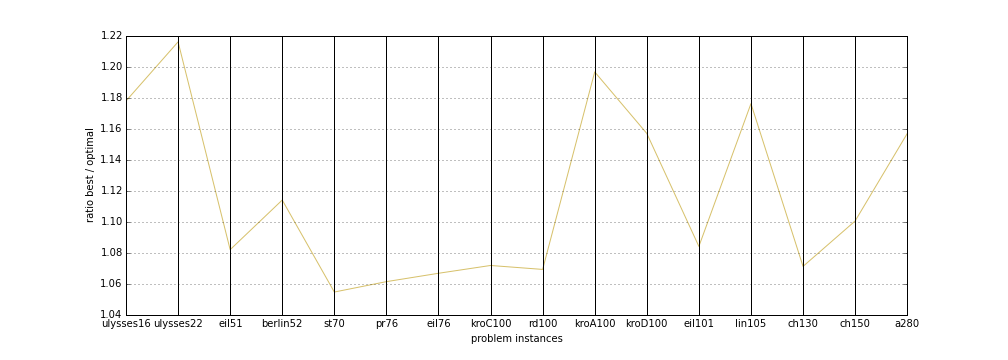
\includegraphics[scale=0.4]{figs/ratios_mc}
	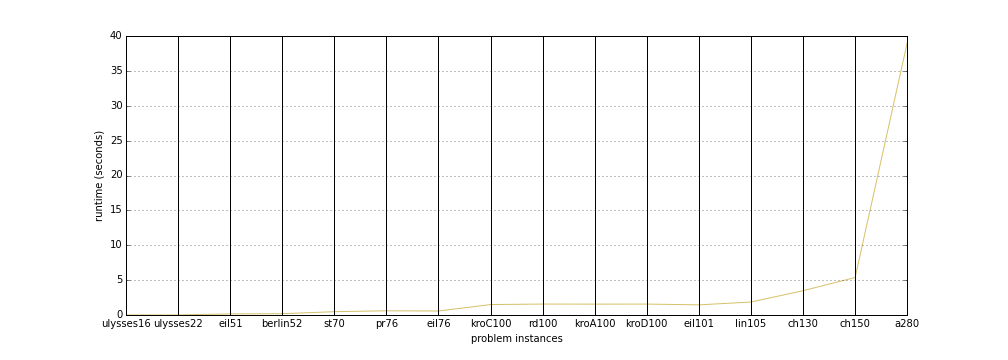
\includegraphics[scale=0.4]{figs/runtimes_mc}
	\caption{\small Distance ratio and runtime of obtained solution against optimal known solution. The problems are arranged by the number of clients to visit in increasing order from left to right. We can see that the quality of the solutions is quite good, especially for a baseline and the runtime isn't so bad (considering 5 different solutions were generated for each problem).}
	\label{baseline_results}
\end{figure}


\newpage
\subsubsection{Elastic Net}

\begin{figure}[!htb]
	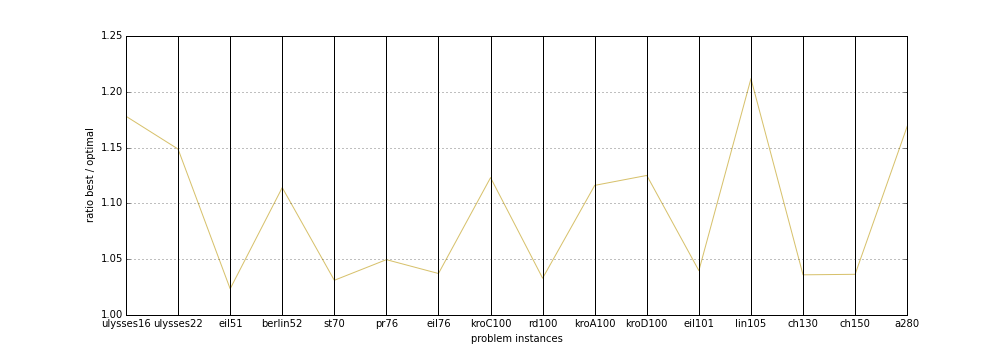
\includegraphics[scale=0.4]{figs/ratios}
	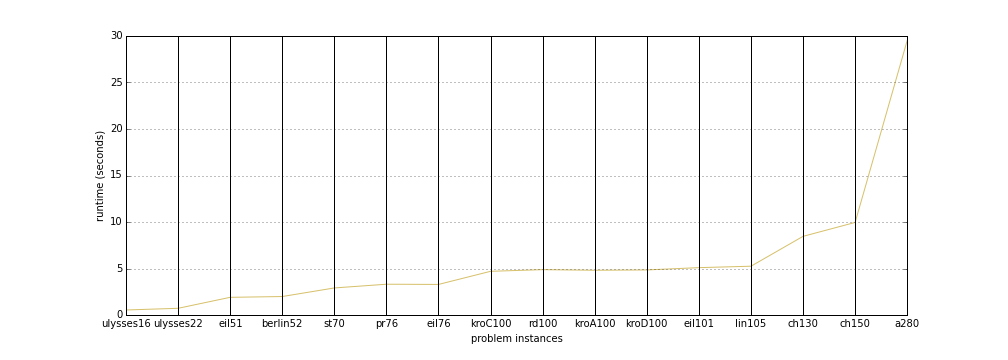
\includegraphics[scale=0.4]{figs/runtimes}
	\caption{\small Distance ratio and runtime of obtained solution against optimal known solution. The problems are arranged by the number of clients to visit in increasing order from left to right. We can see that the number of clients doesn't seem to influence the relative performance. The results are quite good, going from 2\% to 18\% of the optimal values. Full solutions can be visualized in \cref{TSPLIB_solutions}.}

\label{en_results}
\end{figure}



\newpage
\subsection{Randomly Generated Instances}

Here are the best results obtained for randomly generated problems of size 50, 100 and 200.

\begin{figure}[!htb]
\begin{center}
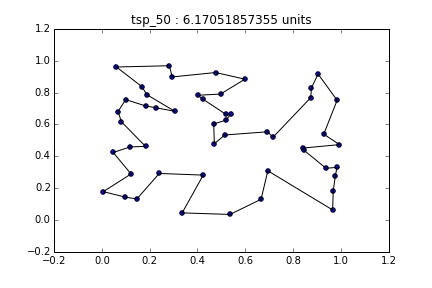
\includegraphics[scale=0.45]{figs/random_tsp_50}
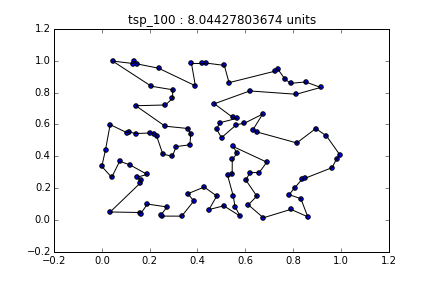
\includegraphics[scale=0.45]{figs/random_tsp_100}
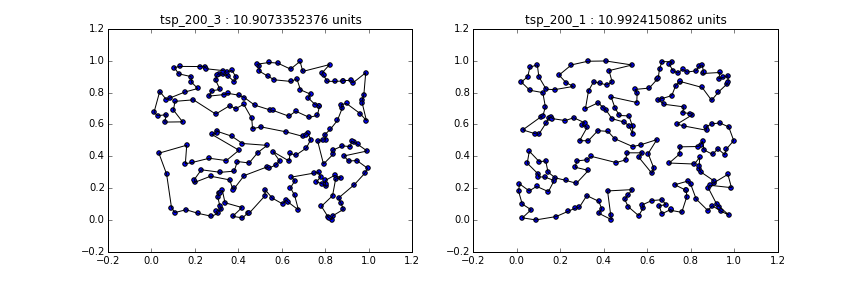
\includegraphics[scale=0.45]{figs/random_tsp_200}

\caption{\small Best solutions to (five different) randomly generated 2D euclidean TSP instances of size 50, 100 and 200. On the left is the baseline and on the right the Elastic Net. Ironically, the baseline is better than the Elastic Net on some instances... Compared to the results from \citep{potvin_ann}, the Elastic Net results are similar for the Elastic Net (5.62, 7.69 and 11.14) and still much better than the Peterson and Soderberg model results (6.61, 8.58, 12.66).}
\label{random_results}
\end{center}
\end{figure}





\newpage
\section{Discussion}
\label{discussion}


\subsection{Challenges}

\subsubsection{Implementation}
The Elastic Net was implemented in a sequential fashion using Cython and Numpy as in the previous homework. All the code is in the IPython Notebook referred in \cref{user_guide}.\newline

The only real implementation detail that was problematic was to avoid exponentiating big negative numbers, that is I initially forgot to transpose the TSP instances in the unit square...


\subsubsection{Parameter Sensitivity}

Unsurprisingly, the algorithm is quite sensitive to the parameters used. The basic parameters were the following.

\begin{itemize}
	\item $M$ = 2.5N
	\item radius of initial net = 0.01
	\item $\alpha$ = 0.2
	\item $\beta$ = 2.0
	\item $K$ = 0.2
	\item $K$ is decreased 1\% every 25 iterations
	\item lowest $K$ = 0.01
	\item 2500 iterations
\end{itemize}

The Elastic Net is quite sensitive to most of these parameters. It is certainly very sensitive to the ratio of the two forces involved in the update of the network ($\alpha$, $\beta$ and $K$), as it drives the net towards a minima.\newline

I didn't play too much with the parameters, but it seems that choosing the decay of K is quite important while the number of iterations doesn't make much of a difference as long as the net has converged a bit. An additional effort could have been made to use convergence as a stopping criteria, but that would imply a risk of prematurely stopping.

\subsection{Performance Analysis}

First of all, the baseline method was surprisingly good. The major computational cost comes from the 2-opt descent which is $O(n^2)$ on the size of the problem instance, but it still manages to finish really fast. Its speed and quality of solutions was much better than expected (\cref{baseline_results,random_results}).\newline


The Elastic Net algorithm was also very fast and should be much faster given a parallel implementation. Also, since the choice of parameters is important, it isn't clear that a bigger number of iterations with slower decay of K is better (the opposite was actually observed on some instances).

The performance on TSPLIB instances is generally better than the baseline (\cref{en_results}) and comes close to optimal for some instances.
The quality of the solutions for randomly generated instances (\cref{random_results}) is also good and very similar to the expected values from \citep{potvin_ann}.




\section{Conclusion}
\label{conclusion}

The Elastic Net approach to the TSP is an interesting idea with some nice theoretical guarantees \citep{en_theoretical_analysis}. It seems generally reliable and efficient and I find it more intuitive than the self-organizing map.\newline


I am still surprised that the baseline method yielded such good results given its simplicity, but I believe that it doesn't have the potential to scale as well as the Elastic Net should.



\bibliographystyle{plain}
\bibliography{dev3}


\newpage
\section{Supplementary Materials}

\subsection{User Guide}
\label{user_guide}

The following section should help with verification of the results and repeatability.\newline

The language used is a mix of python and cython, an optimising compiler that allows static typing and generates C code.


\subsubsection{Working Environment}
All computational results obtained in this work should be repeatable given a suitable python environment. The particular dependencies of this work are the Cython, Numpy, IPython and Seaborn along with standard python environment.\newline

The following python environment was used:

\begin{verbatim}
CPython 2.7.9
ipython 2.2.0

numpy 1.9.2
cython 0.21
ipython 2.2.0

compiler   : GCC 4.4.7 20120313 (Red Hat 4.4.7-1)
system     : Linux
release    : 3.13.0-46-generic
machine    : x86_64
processor  : x86_64
CPU cores  : 4
interpreter: 64bit

\end{verbatim}

As of now, my personal recommendation is to use the excellent \href{http://continuum.io/downloads}{Anaconda python distribution} from Continuum Analytics.


\subsubsection{Running Computational Results}

All computational results and figures are contained in the form of IPython Notebooks with the hope of allowing repeatability and reproducibility.\newline

If IPython is available on the computer, an IPython Notebook service can be launched from command line by typing "ipython notebook" from the proper directory.\newline

Alternatively, the IPython notebooks can be viewed online if it is reachable from a url using the \href{http://nbviewer.IPython.org/}{nbviewer tool}. This allows viewing a static version of an IPython Notebook.



\subsection{TSPLIB Solutions}
\label{TSPLIB_solutions}
For each of the figures below, the Elastic Net, the corresponding path and the best path obtained from TSPLIB are arranged from left to right.\newline

For more details, all parameters used are specified in the Homework3.ipynb IPython Notebook.

\begin{figure}[!htb]
\begin{center}
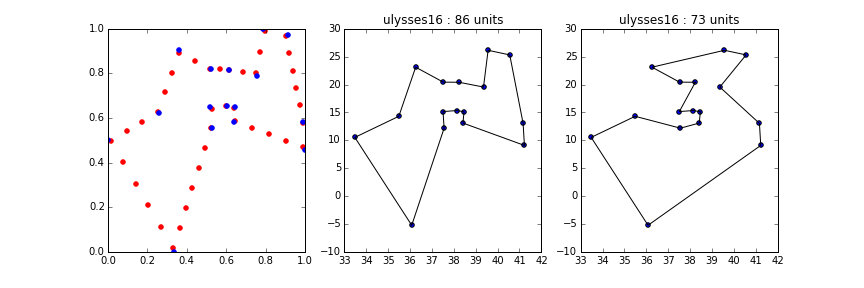
\includegraphics[scale=0.45]{figs/ulysses16}
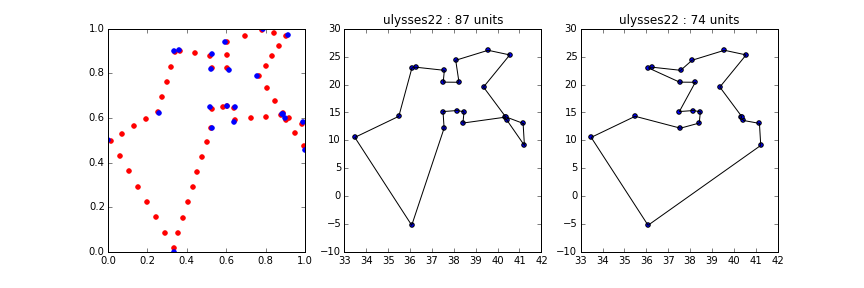
\includegraphics[scale=0.45]{figs/ulysses22}
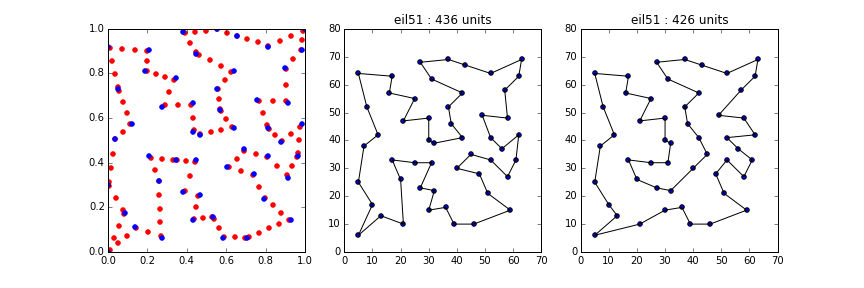
\includegraphics[scale=0.45]{figs/eil51}
 \end{center}
\end{figure}


\begin{figure}[!htb]
\begin{center}
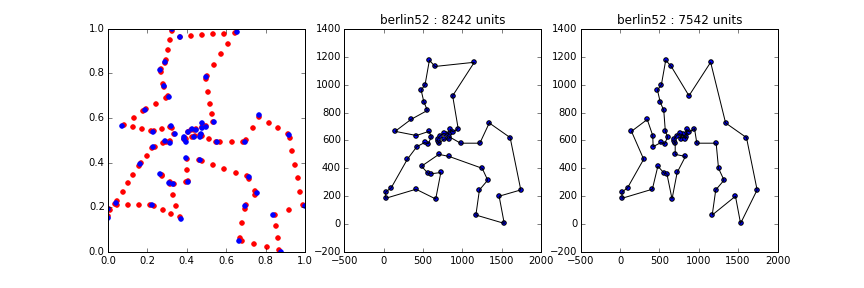
\includegraphics[scale=0.45]{figs/berlin52}
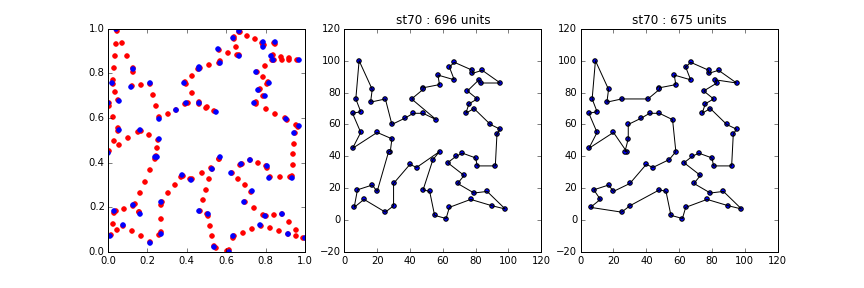
\includegraphics[scale=0.45]{figs/st70}
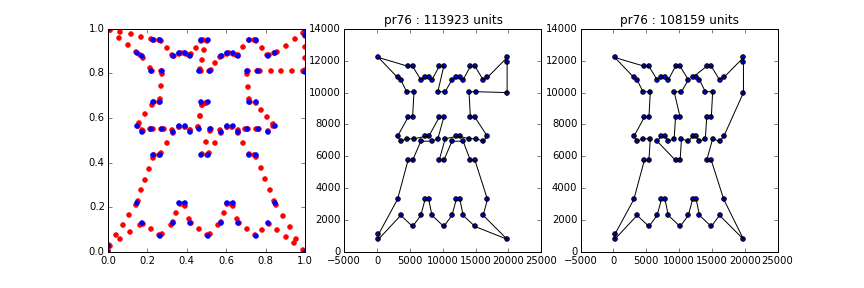
\includegraphics[scale=0.45]{figs/pr76}
 \end{center}
\end{figure}

 


\begin{figure}[!htb]
\begin{center}
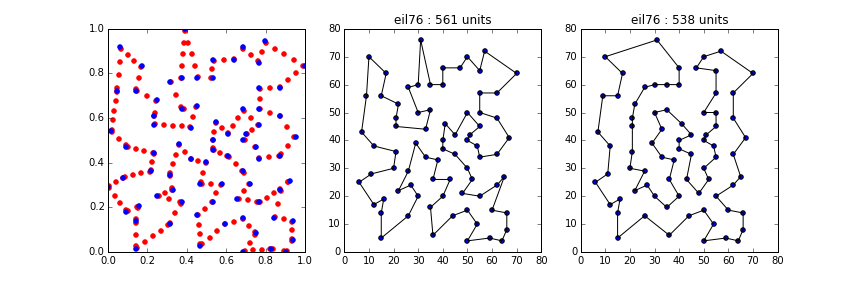
\includegraphics[scale=0.45]{figs/eil76}
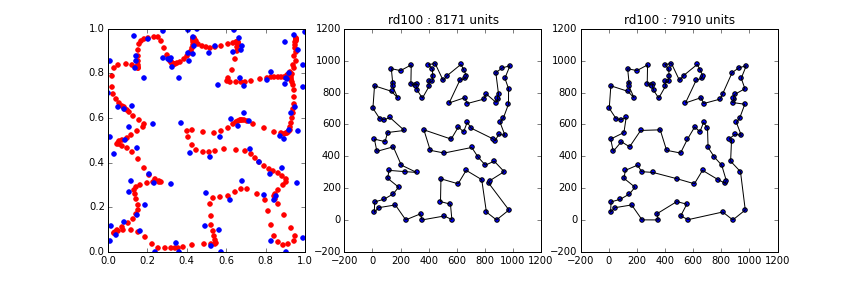
\includegraphics[scale=0.45]{figs/rd100}
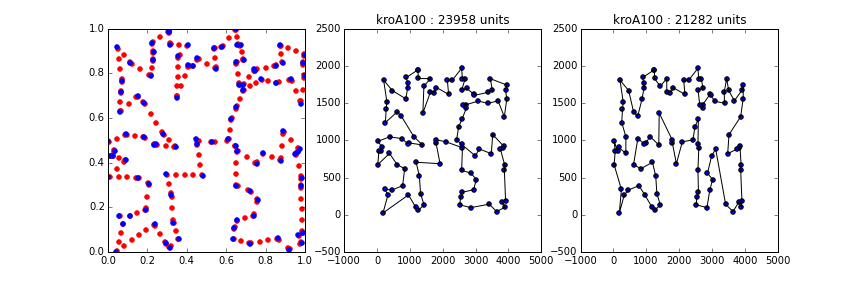
\includegraphics[scale=0.45]{figs/kroA100}

 \end{center}
\end{figure}


\begin{figure}[!htb]
\begin{center}
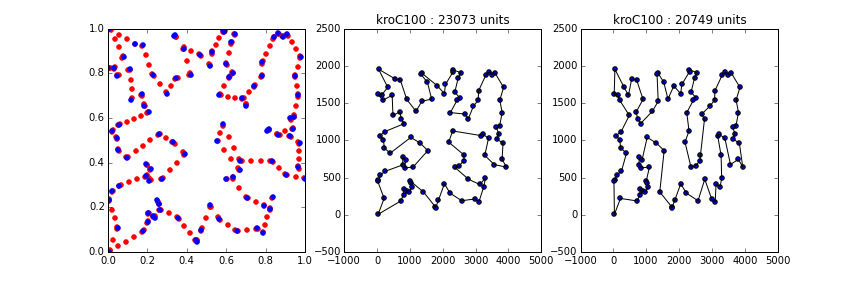
\includegraphics[scale=0.45]{figs/kroC100}
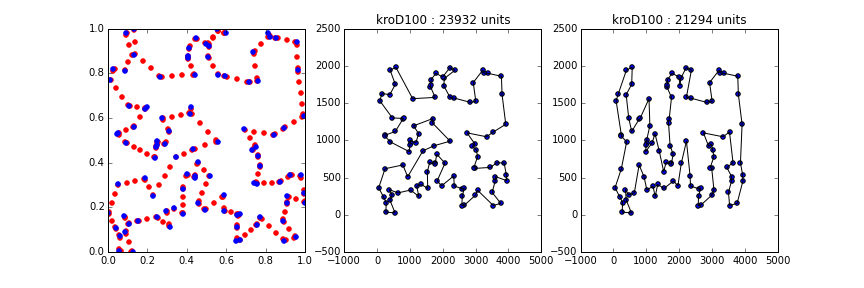
\includegraphics[scale=0.45]{figs/kroD100}
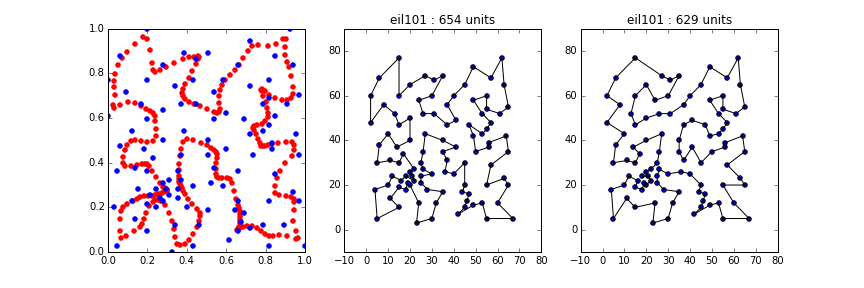
\includegraphics[scale=0.45]{figs/eil101}
 \end{center}
\end{figure}


\begin{figure}[!htb]
\begin{center}
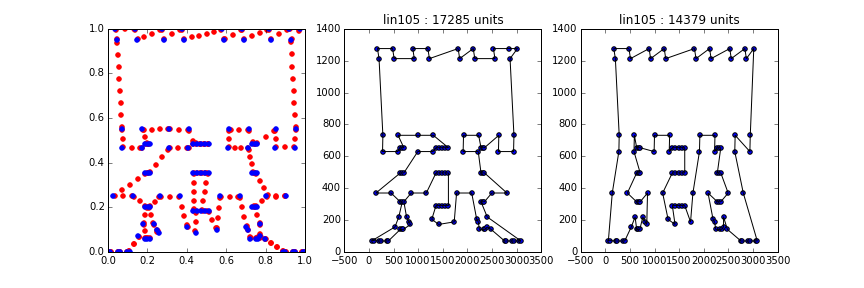
\includegraphics[scale=0.45]{figs/lin105}
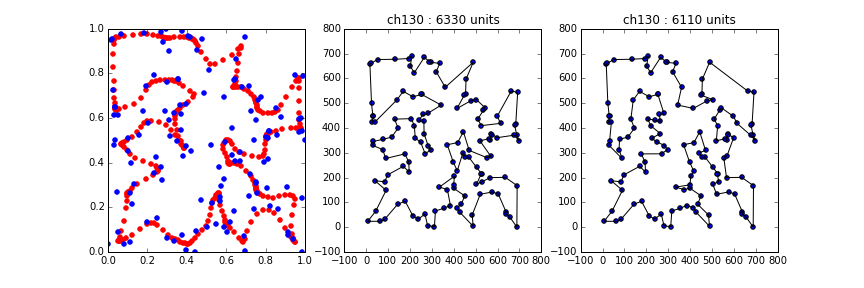
\includegraphics[scale=0.45]{figs/ch130}
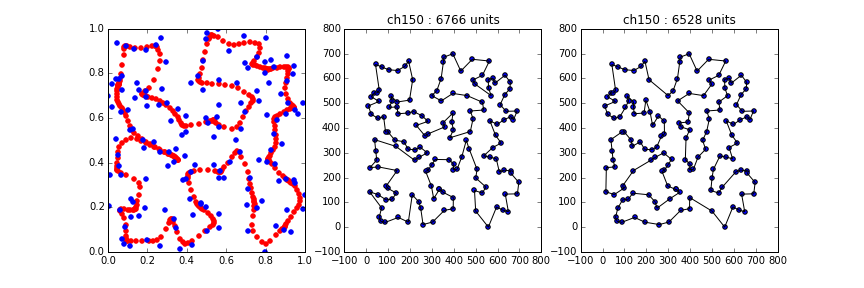
\includegraphics[scale=0.45]{figs/ch150}
 \end{center}
\end{figure}


 


\end{document}


